% Created by tikzDevice version 0.12
% !TEX encoding = UTF-8 Unicode
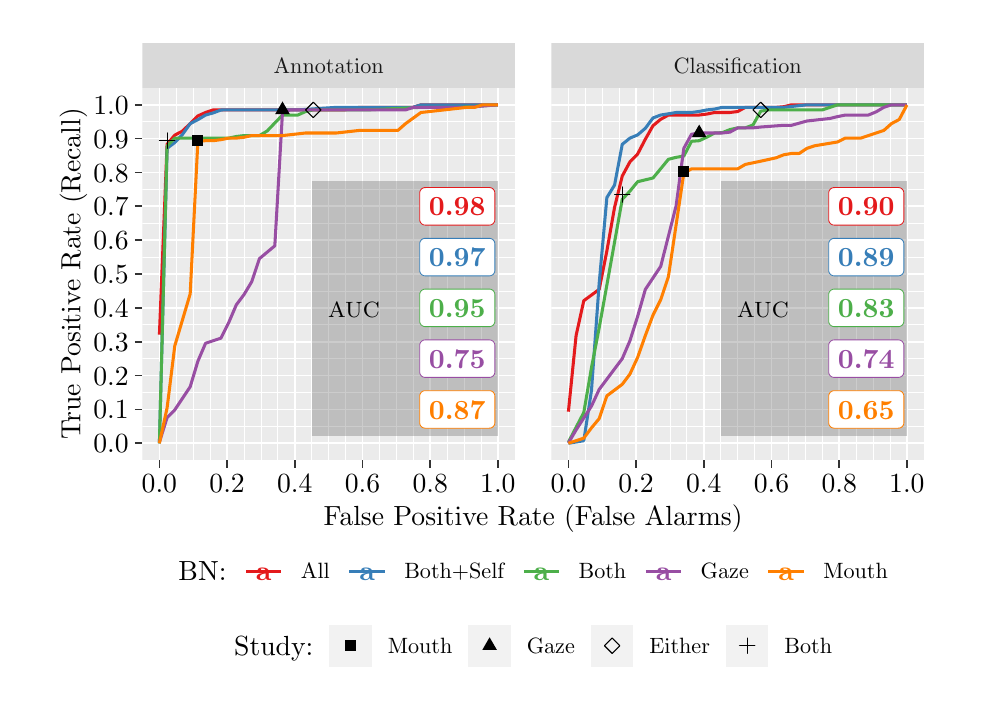
\begin{tikzpicture}[x=1pt,y=1pt]
\definecolor{fillColor}{RGB}{255,255,255}
\path[use as bounding box,fill=fillColor,fill opacity=0.00] (0,0) rectangle (336.00,242.28);
\begin{scope}
\path[clip] (  6.68,  0.00) rectangle (329.32,242.28);
\definecolor{drawColor}{RGB}{255,255,255}
\definecolor{fillColor}{RGB}{255,255,255}

\path[draw=drawColor,line width= 0.6pt,line join=round,line cap=round,fill=fillColor] (  6.68,  0.00) rectangle (329.32,242.28);
\end{scope}
\begin{scope}
\path[clip] ( 41.48, 85.99) rectangle (176.03,220.53);
\definecolor{fillColor}{gray}{0.92}

\path[fill=fillColor] ( 41.48, 85.99) rectangle (176.03,220.53);
\definecolor{drawColor}{RGB}{255,255,255}

\path[draw=drawColor,line width= 0.3pt,line join=round] ( 41.48, 98.22) --
	(176.03, 98.22);

\path[draw=drawColor,line width= 0.3pt,line join=round] ( 41.48,110.45) --
	(176.03,110.45);

\path[draw=drawColor,line width= 0.3pt,line join=round] ( 41.48,122.68) --
	(176.03,122.68);

\path[draw=drawColor,line width= 0.3pt,line join=round] ( 41.48,134.91) --
	(176.03,134.91);

\path[draw=drawColor,line width= 0.3pt,line join=round] ( 41.48,147.14) --
	(176.03,147.14);

\path[draw=drawColor,line width= 0.3pt,line join=round] ( 41.48,159.37) --
	(176.03,159.37);

\path[draw=drawColor,line width= 0.3pt,line join=round] ( 41.48,171.60) --
	(176.03,171.60);

\path[draw=drawColor,line width= 0.3pt,line join=round] ( 41.48,183.84) --
	(176.03,183.84);

\path[draw=drawColor,line width= 0.3pt,line join=round] ( 41.48,196.07) --
	(176.03,196.07);

\path[draw=drawColor,line width= 0.3pt,line join=round] ( 41.48,208.30) --
	(176.03,208.30);

\path[draw=drawColor,line width= 0.3pt,line join=round] ( 53.72, 85.99) --
	( 53.72,220.53);

\path[draw=drawColor,line width= 0.3pt,line join=round] ( 59.83, 85.99) --
	( 59.83,220.53);

\path[draw=drawColor,line width= 0.3pt,line join=round] ( 65.95, 85.99) --
	( 65.95,220.53);

\path[draw=drawColor,line width= 0.3pt,line join=round] ( 78.18, 85.99) --
	( 78.18,220.53);

\path[draw=drawColor,line width= 0.3pt,line join=round] ( 84.29, 85.99) --
	( 84.29,220.53);

\path[draw=drawColor,line width= 0.3pt,line join=round] ( 90.41, 85.99) --
	( 90.41,220.53);

\path[draw=drawColor,line width= 0.3pt,line join=round] (102.64, 85.99) --
	(102.64,220.53);

\path[draw=drawColor,line width= 0.3pt,line join=round] (108.76, 85.99) --
	(108.76,220.53);

\path[draw=drawColor,line width= 0.3pt,line join=round] (114.87, 85.99) --
	(114.87,220.53);

\path[draw=drawColor,line width= 0.3pt,line join=round] (127.10, 85.99) --
	(127.10,220.53);

\path[draw=drawColor,line width= 0.3pt,line join=round] (133.22, 85.99) --
	(133.22,220.53);

\path[draw=drawColor,line width= 0.3pt,line join=round] (139.33, 85.99) --
	(139.33,220.53);

\path[draw=drawColor,line width= 0.3pt,line join=round] (151.57, 85.99) --
	(151.57,220.53);

\path[draw=drawColor,line width= 0.3pt,line join=round] (157.68, 85.99) --
	(157.68,220.53);

\path[draw=drawColor,line width= 0.3pt,line join=round] (163.80, 85.99) --
	(163.80,220.53);

\path[draw=drawColor,line width= 0.6pt,line join=round] ( 41.48, 92.10) --
	(176.03, 92.10);

\path[draw=drawColor,line width= 0.6pt,line join=round] ( 41.48,104.33) --
	(176.03,104.33);

\path[draw=drawColor,line width= 0.6pt,line join=round] ( 41.48,116.56) --
	(176.03,116.56);

\path[draw=drawColor,line width= 0.6pt,line join=round] ( 41.48,128.80) --
	(176.03,128.80);

\path[draw=drawColor,line width= 0.6pt,line join=round] ( 41.48,141.03) --
	(176.03,141.03);

\path[draw=drawColor,line width= 0.6pt,line join=round] ( 41.48,153.26) --
	(176.03,153.26);

\path[draw=drawColor,line width= 0.6pt,line join=round] ( 41.48,165.49) --
	(176.03,165.49);

\path[draw=drawColor,line width= 0.6pt,line join=round] ( 41.48,177.72) --
	(176.03,177.72);

\path[draw=drawColor,line width= 0.6pt,line join=round] ( 41.48,189.95) --
	(176.03,189.95);

\path[draw=drawColor,line width= 0.6pt,line join=round] ( 41.48,202.18) --
	(176.03,202.18);

\path[draw=drawColor,line width= 0.6pt,line join=round] ( 41.48,214.41) --
	(176.03,214.41);

\path[draw=drawColor,line width= 0.6pt,line join=round] ( 47.60, 85.99) --
	( 47.60,220.53);

\path[draw=drawColor,line width= 0.6pt,line join=round] ( 72.06, 85.99) --
	( 72.06,220.53);

\path[draw=drawColor,line width= 0.6pt,line join=round] ( 96.52, 85.99) --
	( 96.52,220.53);

\path[draw=drawColor,line width= 0.6pt,line join=round] (120.99, 85.99) --
	(120.99,220.53);

\path[draw=drawColor,line width= 0.6pt,line join=round] (145.45, 85.99) --
	(145.45,220.53);

\path[draw=drawColor,line width= 0.6pt,line join=round] (169.91, 85.99) --
	(169.91,220.53);
\definecolor{fillColor}{RGB}{89,89,89}

\path[fill=fillColor,fill opacity=0.30] (102.64, 94.85) rectangle (169.91,186.89);
\definecolor{drawColor}{RGB}{0,0,0}

\node[text=drawColor,anchor=base,inner sep=0pt, outer sep=0pt, scale=  1.00] at (117.93,137.57) {\footnotesize{AUC}};
\definecolor{drawColor}{RGB}{255,127,0}
\definecolor{fillColor}{RGB}{255,255,255}

\path[draw=drawColor,line width= 0.3pt,line join=round,line cap=round,fill=fillColor] (143.65, 97.56) --
	(166.82, 97.56) --
	(166.74, 97.56) --
	(167.06, 97.57) --
	(167.37, 97.63) --
	(167.67, 97.75) --
	(167.95, 97.91) --
	(168.20, 98.11) --
	(168.41, 98.35) --
	(168.58, 98.62) --
	(168.71, 98.91) --
	(168.78, 99.22) --
	(168.81, 99.54) --
	(168.81, 99.54) --
	(168.81,109.12) --
	(168.81,109.12) --
	(168.78,109.44) --
	(168.71,109.75) --
	(168.58,110.05) --
	(168.41,110.32) --
	(168.20,110.56) --
	(167.95,110.76) --
	(167.67,110.92) --
	(167.37,111.03) --
	(167.06,111.10) --
	(166.82,111.11) --
	(143.65,111.11) --
	(143.89,111.10) --
	(143.57,111.11) --
	(143.25,111.07) --
	(142.94,110.98) --
	(142.66,110.84) --
	(142.39,110.66) --
	(142.16,110.44) --
	(141.97,110.18) --
	(141.82,109.90) --
	(141.72,109.60) --
	(141.67,109.28) --
	(141.66,109.12) --
	(141.66, 99.54) --
	(141.67, 99.70) --
	(141.67, 99.38) --
	(141.72, 99.07) --
	(141.82, 98.76) --
	(141.97, 98.48) --
	(142.16, 98.23) --
	(142.39, 98.00) --
	(142.66, 97.82) --
	(142.94, 97.69) --
	(143.25, 97.60) --
	(143.57, 97.56) --
	cycle;
\end{scope}
\begin{scope}
\path[clip] ( 41.48, 85.99) rectangle (176.03,220.53);
\definecolor{drawColor}{RGB}{255,127,0}

\node[text=drawColor,anchor=base,inner sep=0pt, outer sep=0pt, scale=  1.00] at (155.24,100.87) {\bfseries 0.87};
\definecolor{drawColor}{RGB}{152,78,163}
\definecolor{fillColor}{RGB}{255,255,255}

\path[draw=drawColor,line width= 0.3pt,line join=round,line cap=round,fill=fillColor] (143.65,115.90) --
	(166.82,115.90) --
	(166.74,115.90) --
	(167.06,115.92) --
	(167.37,115.98) --
	(167.67,116.10) --
	(167.95,116.25) --
	(168.20,116.46) --
	(168.41,116.70) --
	(168.58,116.97) --
	(168.71,117.26) --
	(168.78,117.57) --
	(168.81,117.89) --
	(168.81,117.89) --
	(168.81,127.47) --
	(168.81,127.47) --
	(168.78,127.79) --
	(168.71,128.10) --
	(168.58,128.39) --
	(168.41,128.66) --
	(168.20,128.90) --
	(167.95,129.10) --
	(167.67,129.26) --
	(167.37,129.38) --
	(167.06,129.44) --
	(166.82,129.46) --
	(143.65,129.46) --
	(143.89,129.44) --
	(143.57,129.45) --
	(143.25,129.42) --
	(142.94,129.33) --
	(142.66,129.19) --
	(142.39,129.01) --
	(142.16,128.79) --
	(141.97,128.53) --
	(141.82,128.25) --
	(141.72,127.94) --
	(141.67,127.63) --
	(141.66,127.47) --
	(141.66,117.89) --
	(141.67,118.05) --
	(141.67,117.73) --
	(141.72,117.41) --
	(141.82,117.11) --
	(141.97,116.83) --
	(142.16,116.57) --
	(142.39,116.35) --
	(142.66,116.17) --
	(142.94,116.03) --
	(143.25,115.94) --
	(143.57,115.90) --
	cycle;
\end{scope}
\begin{scope}
\path[clip] ( 41.48, 85.99) rectangle (176.03,220.53);
\definecolor{drawColor}{RGB}{152,78,163}

\node[text=drawColor,anchor=base,inner sep=0pt, outer sep=0pt, scale=  1.00] at (155.24,119.22) {\bfseries 0.75};
\definecolor{drawColor}{RGB}{77,175,74}
\definecolor{fillColor}{RGB}{255,255,255}

\path[draw=drawColor,line width= 0.3pt,line join=round,line cap=round,fill=fillColor] (143.65,134.25) --
	(166.82,134.25) --
	(166.74,134.25) --
	(167.06,134.26) --
	(167.37,134.33) --
	(167.67,134.44) --
	(167.95,134.60) --
	(168.20,134.80) --
	(168.41,135.04) --
	(168.58,135.31) --
	(168.71,135.61) --
	(168.78,135.92) --
	(168.81,136.24) --
	(168.81,136.24) --
	(168.81,145.82) --
	(168.81,145.82) --
	(168.78,146.13) --
	(168.71,146.45) --
	(168.58,146.74) --
	(168.41,147.01) --
	(168.20,147.25) --
	(167.95,147.45) --
	(167.67,147.61) --
	(167.37,147.73) --
	(167.06,147.79) --
	(166.82,147.80) --
	(143.65,147.80) --
	(143.89,147.79) --
	(143.57,147.80) --
	(143.25,147.76) --
	(142.94,147.67) --
	(142.66,147.54) --
	(142.39,147.36) --
	(142.16,147.13) --
	(141.97,146.88) --
	(141.82,146.60) --
	(141.72,146.29) --
	(141.67,145.98) --
	(141.66,145.82) --
	(141.66,136.24) --
	(141.67,136.40) --
	(141.67,136.08) --
	(141.72,135.76) --
	(141.82,135.46) --
	(141.97,135.18) --
	(142.16,134.92) --
	(142.39,134.70) --
	(142.66,134.52) --
	(142.94,134.38) --
	(143.25,134.29) --
	(143.57,134.25) --
	cycle;
\end{scope}
\begin{scope}
\path[clip] ( 41.48, 85.99) rectangle (176.03,220.53);
\definecolor{drawColor}{RGB}{77,175,74}

\node[text=drawColor,anchor=base,inner sep=0pt, outer sep=0pt, scale=  1.00] at (155.24,137.56) {\bfseries 0.95};
\definecolor{drawColor}{RGB}{55,126,184}
\definecolor{fillColor}{RGB}{255,255,255}

\path[draw=drawColor,line width= 0.3pt,line join=round,line cap=round,fill=fillColor] (143.65,152.60) --
	(166.82,152.60) --
	(166.74,152.60) --
	(167.06,152.61) --
	(167.37,152.68) --
	(167.67,152.79) --
	(167.95,152.95) --
	(168.20,153.15) --
	(168.41,153.39) --
	(168.58,153.66) --
	(168.71,153.95) --
	(168.78,154.27) --
	(168.81,154.58) --
	(168.81,154.58) --
	(168.81,164.16) --
	(168.81,164.16) --
	(168.78,164.48) --
	(168.71,164.79) --
	(168.58,165.09) --
	(168.41,165.36) --
	(168.20,165.60) --
	(167.95,165.80) --
	(167.67,165.96) --
	(167.37,166.07) --
	(167.06,166.14) --
	(166.82,166.15) --
	(143.65,166.15) --
	(143.89,166.14) --
	(143.57,166.15) --
	(143.25,166.11) --
	(142.94,166.02) --
	(142.66,165.88) --
	(142.39,165.70) --
	(142.16,165.48) --
	(141.97,165.23) --
	(141.82,164.94) --
	(141.72,164.64) --
	(141.67,164.32) --
	(141.66,164.16) --
	(141.66,154.58) --
	(141.67,154.74) --
	(141.67,154.42) --
	(141.72,154.11) --
	(141.82,153.81) --
	(141.97,153.52) --
	(142.16,153.27) --
	(142.39,153.04) --
	(142.66,152.86) --
	(142.94,152.73) --
	(143.25,152.64) --
	(143.57,152.60) --
	cycle;
\end{scope}
\begin{scope}
\path[clip] ( 41.48, 85.99) rectangle (176.03,220.53);
\definecolor{drawColor}{RGB}{55,126,184}

\node[text=drawColor,anchor=base,inner sep=0pt, outer sep=0pt, scale=  1.00] at (155.24,155.91) {\bfseries 0.97};
\definecolor{drawColor}{RGB}{228,26,28}
\definecolor{fillColor}{RGB}{255,255,255}

\path[draw=drawColor,line width= 0.3pt,line join=round,line cap=round,fill=fillColor] (143.65,170.94) --
	(166.82,170.94) --
	(166.74,170.95) --
	(167.06,170.96) --
	(167.37,171.02) --
	(167.67,171.14) --
	(167.95,171.30) --
	(168.20,171.50) --
	(168.41,171.74) --
	(168.58,172.01) --
	(168.71,172.30) --
	(168.78,172.61) --
	(168.81,172.93) --
	(168.81,172.93) --
	(168.81,182.51) --
	(168.81,182.51) --
	(168.78,182.83) --
	(168.71,183.14) --
	(168.58,183.43) --
	(168.41,183.70) --
	(168.20,183.94) --
	(167.95,184.15) --
	(167.67,184.31) --
	(167.37,184.42) --
	(167.06,184.48) --
	(166.82,184.50) --
	(143.65,184.50) --
	(143.89,184.48) --
	(143.57,184.50) --
	(143.25,184.46) --
	(142.94,184.37) --
	(142.66,184.23) --
	(142.39,184.05) --
	(142.16,183.83) --
	(141.97,183.57) --
	(141.82,183.29) --
	(141.72,182.99) --
	(141.67,182.67) --
	(141.66,182.51) --
	(141.66,172.93) --
	(141.67,173.09) --
	(141.67,172.77) --
	(141.72,172.46) --
	(141.82,172.15) --
	(141.97,171.87) --
	(142.16,171.61) --
	(142.39,171.39) --
	(142.66,171.21) --
	(142.94,171.07) --
	(143.25,170.98) --
	(143.57,170.95) --
	cycle;
\end{scope}
\begin{scope}
\path[clip] ( 41.48, 85.99) rectangle (176.03,220.53);
\definecolor{drawColor}{RGB}{228,26,28}

\node[text=drawColor,anchor=base,inner sep=0pt, outer sep=0pt, scale=  1.00] at (155.24,174.26) {\bfseries 0.98};

\path[draw=drawColor,line width= 1.1pt,line join=round] ( 47.60,131.33) --
	( 50.38,200.17) --
	( 53.16,203.45) --
	( 55.94,204.92) --
	( 58.72,207.62) --
	( 61.50,210.40) --
	( 64.28,211.63) --
	( 67.06,212.56) --
	( 69.84,212.56) --
	( 72.62,212.56) --
	( 75.40,212.56) --
	( 78.18,212.56) --
	( 86.52,212.56) --
	( 89.30,212.56) --
	( 92.08,212.56) --
	( 94.86,212.56) --
	( 97.64,212.56) --
	(105.98,212.56) --
	(108.76,212.56) --
	(114.32,212.56) --
	(119.88,213.49) --
	(128.22,213.49) --
	(139.33,213.49) --
	(142.11,214.41) --
	(144.89,214.41) --
	(169.91,214.41);
\definecolor{drawColor}{RGB}{55,126,184}

\path[draw=drawColor,line width= 1.1pt,line join=round] ( 47.60, 92.10) --
	( 50.38,198.67) --
	( 53.16,200.78) --
	( 55.94,203.70) --
	( 58.72,207.60) --
	( 61.50,209.03) --
	( 64.28,210.71) --
	( 67.06,211.48) --
	( 69.84,212.53) --
	( 72.62,212.56) --
	( 75.40,212.56) --
	( 80.96,212.56) --
	( 83.74,212.56) --
	( 86.52,212.56) --
	( 97.64,212.56) --
	(111.54,213.49) --
	(125.44,213.49) --
	(128.22,213.49) --
	(130.99,213.49) --
	(136.55,213.49) --
	(139.33,213.49) --
	(142.11,214.41) --
	(169.91,214.41);
\definecolor{drawColor}{RGB}{77,175,74}

\path[draw=drawColor,line width= 1.1pt,line join=round] ( 47.60, 92.10) --
	( 50.38,199.50) --
	( 53.16,202.37) --
	( 55.94,202.37) --
	( 58.72,202.37) --
	( 67.06,202.37) --
	( 69.84,202.37) --
	( 72.62,202.37) --
	( 75.40,202.95) --
	( 78.18,203.29) --
	( 80.96,203.29) --
	( 83.74,203.29) --
	( 86.52,204.92) --
	( 89.30,207.84) --
	( 92.08,210.71) --
	( 94.86,210.71) --
	( 97.64,210.71) --
	(100.42,211.97) --
	(103.20,212.56) --
	(111.54,212.56) --
	(122.66,212.56) --
	(142.11,213.49) --
	(156.01,213.49) --
	(169.91,214.41);
\definecolor{drawColor}{RGB}{152,78,163}

\path[draw=drawColor,line width= 1.1pt,line join=round] ( 47.60, 92.49) --
	( 50.38,101.37) --
	( 53.16,104.15) --
	( 58.72,112.49) --
	( 61.50,121.75) --
	( 64.28,128.24) --
	( 69.84,130.09) --
	( 72.62,135.65) --
	( 75.40,142.14) --
	( 78.18,145.85) --
	( 80.96,150.48) --
	( 83.74,158.82) --
	( 89.30,163.45) --
	( 92.08,211.73) --
	( 94.86,212.56) --
	( 97.64,212.56) --
	(103.20,212.56) --
	(105.98,212.56) --
	(111.54,212.56) --
	(117.10,212.56) --
	(122.66,212.56) --
	(125.44,212.56) --
	(128.22,212.56) --
	(133.77,212.56) --
	(136.55,212.56) --
	(139.33,213.49) --
	(142.11,213.49) --
	(147.67,213.49) --
	(153.23,213.49) --
	(158.79,213.49) --
	(164.35,213.95) --
	(169.91,214.41);
\definecolor{drawColor}{RGB}{255,127,0}

\path[draw=drawColor,line width= 1.1pt,line join=round] ( 47.60, 92.10) --
	( 50.38,104.89) --
	( 53.16,127.31) --
	( 58.72,146.08) --
	( 61.50,201.22) --
	( 64.28,201.44) --
	( 67.06,201.44) --
	( 69.84,201.81) --
	( 72.62,202.37) --
	( 75.40,202.37) --
	( 78.18,202.68) --
	( 80.96,203.29) --
	( 83.74,203.29) --
	( 86.52,203.29) --
	( 92.08,203.29) --
	(100.42,204.22) --
	(103.20,204.22) --
	(105.98,204.22) --
	(108.76,204.22) --
	(111.54,204.22) --
	(119.88,205.15) --
	(122.66,205.15) --
	(125.44,205.15) --
	(128.22,205.15) --
	(130.99,205.15) --
	(133.77,205.15) --
	(136.55,207.60) --
	(142.11,211.63) --
	(150.45,212.56) --
	(158.79,213.49) --
	(161.57,213.49) --
	(164.35,214.41) --
	(167.13,214.41) --
	(169.91,214.41);
\definecolor{fillColor}{RGB}{0,0,0}

\path[fill=fillColor] ( 92.08,215.61) --
	( 94.72,211.04) --
	( 89.43,211.04) --
	cycle;

\path[fill=fillColor] ( 59.54,199.48) --
	( 63.46,199.48) --
	( 63.46,203.40) --
	( 59.54,203.40) --
	cycle;
\definecolor{drawColor}{RGB}{0,0,0}

\path[draw=drawColor,line width= 0.4pt,line join=round,line cap=round] ( 47.60,201.44) -- ( 53.15,201.44);

\path[draw=drawColor,line width= 0.4pt,line join=round,line cap=round] ( 50.38,198.67) -- ( 50.38,204.22);

\path[draw=drawColor,line width= 0.4pt,line join=round,line cap=round] (100.42,212.56) --
	(103.20,215.34) --
	(105.97,212.56) --
	(103.20,209.79) --
	(100.42,212.56);
\end{scope}
\begin{scope}
\path[clip] (189.28, 85.99) rectangle (323.82,220.53);
\definecolor{fillColor}{gray}{0.92}

\path[fill=fillColor] (189.28, 85.99) rectangle (323.82,220.53);
\definecolor{drawColor}{RGB}{255,255,255}

\path[draw=drawColor,line width= 0.3pt,line join=round] (189.28, 98.22) --
	(323.82, 98.22);

\path[draw=drawColor,line width= 0.3pt,line join=round] (189.28,110.45) --
	(323.82,110.45);

\path[draw=drawColor,line width= 0.3pt,line join=round] (189.28,122.68) --
	(323.82,122.68);

\path[draw=drawColor,line width= 0.3pt,line join=round] (189.28,134.91) --
	(323.82,134.91);

\path[draw=drawColor,line width= 0.3pt,line join=round] (189.28,147.14) --
	(323.82,147.14);

\path[draw=drawColor,line width= 0.3pt,line join=round] (189.28,159.37) --
	(323.82,159.37);

\path[draw=drawColor,line width= 0.3pt,line join=round] (189.28,171.60) --
	(323.82,171.60);

\path[draw=drawColor,line width= 0.3pt,line join=round] (189.28,183.84) --
	(323.82,183.84);

\path[draw=drawColor,line width= 0.3pt,line join=round] (189.28,196.07) --
	(323.82,196.07);

\path[draw=drawColor,line width= 0.3pt,line join=round] (189.28,208.30) --
	(323.82,208.30);

\path[draw=drawColor,line width= 0.3pt,line join=round] (201.51, 85.99) --
	(201.51,220.53);

\path[draw=drawColor,line width= 0.3pt,line join=round] (207.62, 85.99) --
	(207.62,220.53);

\path[draw=drawColor,line width= 0.3pt,line join=round] (213.74, 85.99) --
	(213.74,220.53);

\path[draw=drawColor,line width= 0.3pt,line join=round] (225.97, 85.99) --
	(225.97,220.53);

\path[draw=drawColor,line width= 0.3pt,line join=round] (232.09, 85.99) --
	(232.09,220.53);

\path[draw=drawColor,line width= 0.3pt,line join=round] (238.20, 85.99) --
	(238.20,220.53);

\path[draw=drawColor,line width= 0.3pt,line join=round] (250.43, 85.99) --
	(250.43,220.53);

\path[draw=drawColor,line width= 0.3pt,line join=round] (256.55, 85.99) --
	(256.55,220.53);

\path[draw=drawColor,line width= 0.3pt,line join=round] (262.67, 85.99) --
	(262.67,220.53);

\path[draw=drawColor,line width= 0.3pt,line join=round] (274.90, 85.99) --
	(274.90,220.53);

\path[draw=drawColor,line width= 0.3pt,line join=round] (281.01, 85.99) --
	(281.01,220.53);

\path[draw=drawColor,line width= 0.3pt,line join=round] (287.13, 85.99) --
	(287.13,220.53);

\path[draw=drawColor,line width= 0.3pt,line join=round] (299.36, 85.99) --
	(299.36,220.53);

\path[draw=drawColor,line width= 0.3pt,line join=round] (305.47, 85.99) --
	(305.47,220.53);

\path[draw=drawColor,line width= 0.3pt,line join=round] (311.59, 85.99) --
	(311.59,220.53);

\path[draw=drawColor,line width= 0.6pt,line join=round] (189.28, 92.10) --
	(323.82, 92.10);

\path[draw=drawColor,line width= 0.6pt,line join=round] (189.28,104.33) --
	(323.82,104.33);

\path[draw=drawColor,line width= 0.6pt,line join=round] (189.28,116.56) --
	(323.82,116.56);

\path[draw=drawColor,line width= 0.6pt,line join=round] (189.28,128.80) --
	(323.82,128.80);

\path[draw=drawColor,line width= 0.6pt,line join=round] (189.28,141.03) --
	(323.82,141.03);

\path[draw=drawColor,line width= 0.6pt,line join=round] (189.28,153.26) --
	(323.82,153.26);

\path[draw=drawColor,line width= 0.6pt,line join=round] (189.28,165.49) --
	(323.82,165.49);

\path[draw=drawColor,line width= 0.6pt,line join=round] (189.28,177.72) --
	(323.82,177.72);

\path[draw=drawColor,line width= 0.6pt,line join=round] (189.28,189.95) --
	(323.82,189.95);

\path[draw=drawColor,line width= 0.6pt,line join=round] (189.28,202.18) --
	(323.82,202.18);

\path[draw=drawColor,line width= 0.6pt,line join=round] (189.28,214.41) --
	(323.82,214.41);

\path[draw=drawColor,line width= 0.6pt,line join=round] (195.39, 85.99) --
	(195.39,220.53);

\path[draw=drawColor,line width= 0.6pt,line join=round] (219.86, 85.99) --
	(219.86,220.53);

\path[draw=drawColor,line width= 0.6pt,line join=round] (244.32, 85.99) --
	(244.32,220.53);

\path[draw=drawColor,line width= 0.6pt,line join=round] (268.78, 85.99) --
	(268.78,220.53);

\path[draw=drawColor,line width= 0.6pt,line join=round] (293.24, 85.99) --
	(293.24,220.53);

\path[draw=drawColor,line width= 0.6pt,line join=round] (317.71, 85.99) --
	(317.71,220.53);
\definecolor{fillColor}{RGB}{89,89,89}

\path[fill=fillColor,fill opacity=0.30] (250.43, 94.85) rectangle (317.71,186.89);
\definecolor{drawColor}{RGB}{0,0,0}

\node[text=drawColor,anchor=base,inner sep=0pt, outer sep=0pt, scale=  1.00] at (265.72,137.57) {\footnotesize{AUC}};
\definecolor{drawColor}{RGB}{255,127,0}
\definecolor{fillColor}{RGB}{255,255,255}

\path[draw=drawColor,line width= 0.3pt,line join=round,line cap=round,fill=fillColor] (291.44, 97.56) --
	(314.61, 97.56) --
	(314.53, 97.56) --
	(314.85, 97.57) --
	(315.17, 97.63) --
	(315.47, 97.75) --
	(315.74, 97.91) --
	(315.99, 98.11) --
	(316.20, 98.35) --
	(316.37, 98.62) --
	(316.50, 98.91) --
	(316.58, 99.22) --
	(316.60, 99.54) --
	(316.60, 99.54) --
	(316.60,109.12) --
	(316.60,109.12) --
	(316.58,109.44) --
	(316.50,109.75) --
	(316.37,110.05) --
	(316.20,110.32) --
	(315.99,110.56) --
	(315.74,110.76) --
	(315.47,110.92) --
	(315.17,111.03) --
	(314.85,111.10) --
	(314.61,111.11) --
	(291.44,111.11) --
	(291.68,111.10) --
	(291.36,111.11) --
	(291.05,111.07) --
	(290.74,110.98) --
	(290.45,110.84) --
	(290.19,110.66) --
	(289.96,110.44) --
	(289.76,110.18) --
	(289.61,109.90) --
	(289.51,109.60) --
	(289.46,109.28) --
	(289.46,109.12) --
	(289.46, 99.54) --
	(289.46, 99.70) --
	(289.46, 99.38) --
	(289.51, 99.07) --
	(289.61, 98.76) --
	(289.76, 98.48) --
	(289.96, 98.23) --
	(290.19, 98.00) --
	(290.45, 97.82) --
	(290.74, 97.69) --
	(291.05, 97.60) --
	(291.36, 97.56) --
	cycle;
\end{scope}
\begin{scope}
\path[clip] (189.28, 85.99) rectangle (323.82,220.53);
\definecolor{drawColor}{RGB}{255,127,0}

\node[text=drawColor,anchor=base,inner sep=0pt, outer sep=0pt, scale=  1.00] at (303.03,100.87) {\bfseries 0.65};
\definecolor{drawColor}{RGB}{152,78,163}
\definecolor{fillColor}{RGB}{255,255,255}

\path[draw=drawColor,line width= 0.3pt,line join=round,line cap=round,fill=fillColor] (291.44,115.90) --
	(314.61,115.90) --
	(314.53,115.90) --
	(314.85,115.92) --
	(315.17,115.98) --
	(315.47,116.10) --
	(315.74,116.25) --
	(315.99,116.46) --
	(316.20,116.70) --
	(316.37,116.97) --
	(316.50,117.26) --
	(316.58,117.57) --
	(316.60,117.89) --
	(316.60,117.89) --
	(316.60,127.47) --
	(316.60,127.47) --
	(316.58,127.79) --
	(316.50,128.10) --
	(316.37,128.39) --
	(316.20,128.66) --
	(315.99,128.90) --
	(315.74,129.10) --
	(315.47,129.26) --
	(315.17,129.38) --
	(314.85,129.44) --
	(314.61,129.46) --
	(291.44,129.46) --
	(291.68,129.44) --
	(291.36,129.45) --
	(291.05,129.42) --
	(290.74,129.33) --
	(290.45,129.19) --
	(290.19,129.01) --
	(289.96,128.79) --
	(289.76,128.53) --
	(289.61,128.25) --
	(289.51,127.94) --
	(289.46,127.63) --
	(289.46,127.47) --
	(289.46,117.89) --
	(289.46,118.05) --
	(289.46,117.73) --
	(289.51,117.41) --
	(289.61,117.11) --
	(289.76,116.83) --
	(289.96,116.57) --
	(290.19,116.35) --
	(290.45,116.17) --
	(290.74,116.03) --
	(291.05,115.94) --
	(291.36,115.90) --
	cycle;
\end{scope}
\begin{scope}
\path[clip] (189.28, 85.99) rectangle (323.82,220.53);
\definecolor{drawColor}{RGB}{152,78,163}

\node[text=drawColor,anchor=base,inner sep=0pt, outer sep=0pt, scale=  1.00] at (303.03,119.22) {\bfseries 0.74};
\definecolor{drawColor}{RGB}{77,175,74}
\definecolor{fillColor}{RGB}{255,255,255}

\path[draw=drawColor,line width= 0.3pt,line join=round,line cap=round,fill=fillColor] (291.44,134.25) --
	(314.61,134.25) --
	(314.53,134.25) --
	(314.85,134.26) --
	(315.17,134.33) --
	(315.47,134.44) --
	(315.74,134.60) --
	(315.99,134.80) --
	(316.20,135.04) --
	(316.37,135.31) --
	(316.50,135.61) --
	(316.58,135.92) --
	(316.60,136.24) --
	(316.60,136.24) --
	(316.60,145.82) --
	(316.60,145.82) --
	(316.58,146.13) --
	(316.50,146.45) --
	(316.37,146.74) --
	(316.20,147.01) --
	(315.99,147.25) --
	(315.74,147.45) --
	(315.47,147.61) --
	(315.17,147.73) --
	(314.85,147.79) --
	(314.61,147.80) --
	(291.44,147.80) --
	(291.68,147.79) --
	(291.36,147.80) --
	(291.05,147.76) --
	(290.74,147.67) --
	(290.45,147.54) --
	(290.19,147.36) --
	(289.96,147.13) --
	(289.76,146.88) --
	(289.61,146.60) --
	(289.51,146.29) --
	(289.46,145.98) --
	(289.46,145.82) --
	(289.46,136.24) --
	(289.46,136.40) --
	(289.46,136.08) --
	(289.51,135.76) --
	(289.61,135.46) --
	(289.76,135.18) --
	(289.96,134.92) --
	(290.19,134.70) --
	(290.45,134.52) --
	(290.74,134.38) --
	(291.05,134.29) --
	(291.36,134.25) --
	cycle;
\end{scope}
\begin{scope}
\path[clip] (189.28, 85.99) rectangle (323.82,220.53);
\definecolor{drawColor}{RGB}{77,175,74}

\node[text=drawColor,anchor=base,inner sep=0pt, outer sep=0pt, scale=  1.00] at (303.03,137.56) {\bfseries 0.83};
\definecolor{drawColor}{RGB}{55,126,184}
\definecolor{fillColor}{RGB}{255,255,255}

\path[draw=drawColor,line width= 0.3pt,line join=round,line cap=round,fill=fillColor] (291.44,152.60) --
	(314.61,152.60) --
	(314.53,152.60) --
	(314.85,152.61) --
	(315.17,152.68) --
	(315.47,152.79) --
	(315.74,152.95) --
	(315.99,153.15) --
	(316.20,153.39) --
	(316.37,153.66) --
	(316.50,153.95) --
	(316.58,154.27) --
	(316.60,154.58) --
	(316.60,154.58) --
	(316.60,164.16) --
	(316.60,164.16) --
	(316.58,164.48) --
	(316.50,164.79) --
	(316.37,165.09) --
	(316.20,165.36) --
	(315.99,165.60) --
	(315.74,165.80) --
	(315.47,165.96) --
	(315.17,166.07) --
	(314.85,166.14) --
	(314.61,166.15) --
	(291.44,166.15) --
	(291.68,166.14) --
	(291.36,166.15) --
	(291.05,166.11) --
	(290.74,166.02) --
	(290.45,165.88) --
	(290.19,165.70) --
	(289.96,165.48) --
	(289.76,165.23) --
	(289.61,164.94) --
	(289.51,164.64) --
	(289.46,164.32) --
	(289.46,164.16) --
	(289.46,154.58) --
	(289.46,154.74) --
	(289.46,154.42) --
	(289.51,154.11) --
	(289.61,153.81) --
	(289.76,153.52) --
	(289.96,153.27) --
	(290.19,153.04) --
	(290.45,152.86) --
	(290.74,152.73) --
	(291.05,152.64) --
	(291.36,152.60) --
	cycle;
\end{scope}
\begin{scope}
\path[clip] (189.28, 85.99) rectangle (323.82,220.53);
\definecolor{drawColor}{RGB}{55,126,184}

\node[text=drawColor,anchor=base,inner sep=0pt, outer sep=0pt, scale=  1.00] at (303.03,155.91) {\bfseries 0.89};
\definecolor{drawColor}{RGB}{228,26,28}
\definecolor{fillColor}{RGB}{255,255,255}

\path[draw=drawColor,line width= 0.3pt,line join=round,line cap=round,fill=fillColor] (291.44,170.94) --
	(314.61,170.94) --
	(314.53,170.95) --
	(314.85,170.96) --
	(315.17,171.02) --
	(315.47,171.14) --
	(315.74,171.30) --
	(315.99,171.50) --
	(316.20,171.74) --
	(316.37,172.01) --
	(316.50,172.30) --
	(316.58,172.61) --
	(316.60,172.93) --
	(316.60,172.93) --
	(316.60,182.51) --
	(316.60,182.51) --
	(316.58,182.83) --
	(316.50,183.14) --
	(316.37,183.43) --
	(316.20,183.70) --
	(315.99,183.94) --
	(315.74,184.15) --
	(315.47,184.31) --
	(315.17,184.42) --
	(314.85,184.48) --
	(314.61,184.50) --
	(291.44,184.50) --
	(291.68,184.48) --
	(291.36,184.50) --
	(291.05,184.46) --
	(290.74,184.37) --
	(290.45,184.23) --
	(290.19,184.05) --
	(289.96,183.83) --
	(289.76,183.57) --
	(289.61,183.29) --
	(289.51,182.99) --
	(289.46,182.67) --
	(289.46,182.51) --
	(289.46,172.93) --
	(289.46,173.09) --
	(289.46,172.77) --
	(289.51,172.46) --
	(289.61,172.15) --
	(289.76,171.87) --
	(289.96,171.61) --
	(290.19,171.39) --
	(290.45,171.21) --
	(290.74,171.07) --
	(291.05,170.98) --
	(291.36,170.95) --
	cycle;
\end{scope}
\begin{scope}
\path[clip] (189.28, 85.99) rectangle (323.82,220.53);
\definecolor{drawColor}{RGB}{228,26,28}

\node[text=drawColor,anchor=base,inner sep=0pt, outer sep=0pt, scale=  1.00] at (303.03,174.26) {\bfseries 0.90};

\path[draw=drawColor,line width= 1.1pt,line join=round] (195.39,103.53) --
	(198.17,131.02) --
	(200.95,143.62) --
	(206.51,147.70) --
	(209.29,161.60) --
	(212.07,177.35) --
	(214.85,188.66) --
	(217.63,193.80) --
	(220.41,196.63) --
	(223.19,201.98) --
	(225.97,206.87) --
	(228.75,209.17) --
	(231.53,210.71) --
	(234.31,210.71) --
	(237.09,210.71) --
	(239.87,210.71) --
	(242.65,210.71) --
	(245.43,211.06) --
	(248.21,211.63) --
	(253.77,211.63) --
	(256.55,211.97) --
	(259.33,213.49) --
	(262.11,213.49) --
	(264.89,213.49) --
	(267.67,213.49) --
	(270.45,213.49) --
	(273.23,213.72) --
	(276.01,214.41) --
	(278.79,214.41) --
	(281.57,214.41) --
	(287.13,214.41) --
	(292.69,214.41) --
	(295.47,214.41) --
	(298.25,214.41) --
	(303.81,214.41) --
	(312.15,214.41) --
	(317.71,214.41);
\definecolor{drawColor}{RGB}{55,126,184}

\path[draw=drawColor,line width= 1.1pt,line join=round] (195.39, 92.10) --
	(200.95, 93.03) --
	(203.73,111.19) --
	(206.51,149.92) --
	(209.29,180.89) --
	(212.07,185.40) --
	(214.85,200.12) --
	(217.63,202.37) --
	(220.41,203.53) --
	(223.19,205.92) --
	(225.97,209.66) --
	(228.75,210.71) --
	(231.53,211.16) --
	(234.31,211.63) --
	(237.09,211.63) --
	(239.87,211.63) --
	(242.65,212.01) --
	(245.43,212.56) --
	(248.21,212.87) --
	(250.99,213.49) --
	(253.77,213.49) --
	(256.55,213.49) --
	(259.33,213.49) --
	(262.11,213.49) --
	(264.89,213.49) --
	(267.67,213.49) --
	(270.45,213.49) --
	(273.23,213.49) --
	(276.01,213.80) --
	(281.57,214.41) --
	(287.13,214.41) --
	(289.91,214.41) --
	(292.69,214.41) --
	(295.47,214.41) --
	(303.81,214.41) --
	(312.15,214.41) --
	(317.71,214.41);
\definecolor{drawColor}{RGB}{77,175,74}

\path[draw=drawColor,line width= 1.1pt,line join=round] (195.39, 92.52) --
	(200.95,103.22) --
	(203.73,119.44) --
	(206.51,133.80) --
	(214.85,180.26) --
	(217.63,183.22) --
	(220.41,186.62) --
	(225.97,187.96) --
	(228.75,191.32) --
	(231.53,194.72) --
	(234.31,195.42) --
	(237.09,195.88) --
	(239.87,201.21) --
	(242.65,201.44) --
	(245.43,202.71) --
	(248.21,204.22) --
	(250.99,204.34) --
	(253.77,205.46) --
	(256.55,206.07) --
	(259.33,206.07) --
	(262.11,207.13) --
	(264.89,212.11) --
	(267.67,212.56) --
	(270.45,212.56) --
	(273.23,212.56) --
	(276.01,212.56) --
	(281.57,212.56) --
	(284.35,212.56) --
	(287.13,212.56) --
	(289.91,213.49) --
	(292.69,214.41) --
	(295.47,214.41) --
	(298.25,214.41) --
	(301.03,214.41) --
	(306.59,214.41) --
	(309.37,214.41) --
	(312.15,214.41) --
	(314.93,214.41) --
	(317.71,214.41);
\definecolor{drawColor}{RGB}{152,78,163}

\path[draw=drawColor,line width= 1.1pt,line join=round] (195.39, 92.18) --
	(198.17, 96.92) --
	(203.73,105.54) --
	(206.51,111.56) --
	(209.29,115.27) --
	(214.85,122.68) --
	(217.63,129.17) --
	(220.41,137.97) --
	(223.19,147.70) --
	(228.75,156.04) --
	(234.31,177.88) --
	(237.09,198.66) --
	(239.87,203.76) --
	(242.65,204.22) --
	(245.43,204.22) --
	(250.99,204.22) --
	(253.77,204.53) --
	(256.55,206.07) --
	(262.11,206.07) --
	(264.89,206.38) --
	(273.23,207.00) --
	(276.01,207.00) --
	(281.57,208.55) --
	(289.91,209.47) --
	(292.69,210.15) --
	(295.47,210.71) --
	(298.25,210.71) --
	(303.81,210.71) --
	(306.59,211.87) --
	(309.37,213.49) --
	(312.15,214.41) --
	(314.93,214.41) --
	(317.71,214.41);
\definecolor{drawColor}{RGB}{255,127,0}

\path[draw=drawColor,line width= 1.1pt,line join=round] (195.39, 92.12) --
	(198.17, 93.03) --
	(200.95, 93.95) --
	(203.73, 97.66) --
	(206.51,101.00) --
	(209.29,109.24) --
	(214.85,113.41) --
	(217.63,117.12) --
	(220.41,123.14) --
	(223.19,131.02) --
	(225.97,138.43) --
	(228.75,143.99) --
	(231.53,152.33) --
	(237.09,189.69) --
	(239.87,191.25) --
	(242.65,191.25) --
	(245.43,191.25) --
	(248.21,191.25) --
	(253.77,191.25) --
	(256.55,191.25) --
	(259.33,192.87) --
	(264.89,194.03) --
	(270.45,195.26) --
	(273.23,196.35) --
	(276.01,196.81) --
	(278.79,196.81) --
	(281.57,198.66) --
	(284.35,199.59) --
	(289.91,200.52) --
	(292.69,200.98) --
	(295.47,202.37) --
	(298.25,202.37) --
	(301.03,202.37) --
	(303.81,203.29) --
	(306.59,204.22) --
	(309.37,205.15) --
	(312.15,207.62) --
	(314.93,209.09) --
	(317.71,214.32);
\definecolor{fillColor}{RGB}{0,0,0}

\path[fill=fillColor] (242.65,207.27) --
	(245.29,202.70) --
	(240.01,202.70) --
	cycle;

\path[fill=fillColor] (235.13,188.36) --
	(239.05,188.36) --
	(239.05,192.28) --
	(235.13,192.28) --
	cycle;
\definecolor{drawColor}{RGB}{0,0,0}

\path[draw=drawColor,line width= 0.4pt,line join=round,line cap=round] (212.08,181.98) -- (217.63,181.98);

\path[draw=drawColor,line width= 0.4pt,line join=round,line cap=round] (214.85,179.21) -- (214.85,184.76);

\path[draw=drawColor,line width= 0.4pt,line join=round,line cap=round] (262.11,212.56) --
	(264.89,215.34) --
	(267.66,212.56) --
	(264.89,209.79) --
	(262.11,212.56);
\end{scope}
\begin{scope}
\path[clip] ( 41.48,220.53) rectangle (176.03,236.78);
\definecolor{fillColor}{gray}{0.85}

\path[fill=fillColor] ( 41.48,220.53) rectangle (176.03,236.78);
\definecolor{drawColor}{gray}{0.10}

\node[text=drawColor,anchor=base,inner sep=0pt, outer sep=0pt, scale=  0.80] at (108.76,225.90) {Annotation};
\end{scope}
\begin{scope}
\path[clip] (189.28,220.53) rectangle (323.82,236.78);
\definecolor{fillColor}{gray}{0.85}

\path[fill=fillColor] (189.28,220.53) rectangle (323.82,236.78);
\definecolor{drawColor}{gray}{0.10}

\node[text=drawColor,anchor=base,inner sep=0pt, outer sep=0pt, scale=  0.80] at (256.55,225.90) {Classification};
\end{scope}
\begin{scope}
\path[clip] (  0.00,  0.00) rectangle (336.00,242.28);
\definecolor{drawColor}{gray}{0.20}

\path[draw=drawColor,line width= 0.6pt,line join=round] ( 47.60, 83.24) --
	( 47.60, 85.99);

\path[draw=drawColor,line width= 0.6pt,line join=round] ( 72.06, 83.24) --
	( 72.06, 85.99);

\path[draw=drawColor,line width= 0.6pt,line join=round] ( 96.52, 83.24) --
	( 96.52, 85.99);

\path[draw=drawColor,line width= 0.6pt,line join=round] (120.99, 83.24) --
	(120.99, 85.99);

\path[draw=drawColor,line width= 0.6pt,line join=round] (145.45, 83.24) --
	(145.45, 85.99);

\path[draw=drawColor,line width= 0.6pt,line join=round] (169.91, 83.24) --
	(169.91, 85.99);
\end{scope}
\begin{scope}
\path[clip] (  0.00,  0.00) rectangle (336.00,242.28);
\definecolor{drawColor}{RGB}{0,0,0}

\node[text=drawColor,anchor=base,inner sep=0pt, outer sep=0pt, scale=  1.00] at ( 47.60, 74.15) {0.0};

\node[text=drawColor,anchor=base,inner sep=0pt, outer sep=0pt, scale=  1.00] at ( 72.06, 74.15) {0.2};

\node[text=drawColor,anchor=base,inner sep=0pt, outer sep=0pt, scale=  1.00] at ( 96.52, 74.15) {0.4};

\node[text=drawColor,anchor=base,inner sep=0pt, outer sep=0pt, scale=  1.00] at (120.99, 74.15) {0.6};

\node[text=drawColor,anchor=base,inner sep=0pt, outer sep=0pt, scale=  1.00] at (145.45, 74.15) {0.8};

\node[text=drawColor,anchor=base,inner sep=0pt, outer sep=0pt, scale=  1.00] at (169.91, 74.15) {1.0};
\end{scope}
\begin{scope}
\path[clip] (  0.00,  0.00) rectangle (336.00,242.28);
\definecolor{drawColor}{gray}{0.20}

\path[draw=drawColor,line width= 0.6pt,line join=round] (195.39, 83.24) --
	(195.39, 85.99);

\path[draw=drawColor,line width= 0.6pt,line join=round] (219.86, 83.24) --
	(219.86, 85.99);

\path[draw=drawColor,line width= 0.6pt,line join=round] (244.32, 83.24) --
	(244.32, 85.99);

\path[draw=drawColor,line width= 0.6pt,line join=round] (268.78, 83.24) --
	(268.78, 85.99);

\path[draw=drawColor,line width= 0.6pt,line join=round] (293.24, 83.24) --
	(293.24, 85.99);

\path[draw=drawColor,line width= 0.6pt,line join=round] (317.71, 83.24) --
	(317.71, 85.99);
\end{scope}
\begin{scope}
\path[clip] (  0.00,  0.00) rectangle (336.00,242.28);
\definecolor{drawColor}{RGB}{0,0,0}

\node[text=drawColor,anchor=base,inner sep=0pt, outer sep=0pt, scale=  1.00] at (195.39, 74.15) {0.0};

\node[text=drawColor,anchor=base,inner sep=0pt, outer sep=0pt, scale=  1.00] at (219.86, 74.15) {0.2};

\node[text=drawColor,anchor=base,inner sep=0pt, outer sep=0pt, scale=  1.00] at (244.32, 74.15) {0.4};

\node[text=drawColor,anchor=base,inner sep=0pt, outer sep=0pt, scale=  1.00] at (268.78, 74.15) {0.6};

\node[text=drawColor,anchor=base,inner sep=0pt, outer sep=0pt, scale=  1.00] at (293.24, 74.15) {0.8};

\node[text=drawColor,anchor=base,inner sep=0pt, outer sep=0pt, scale=  1.00] at (317.71, 74.15) {1.0};
\end{scope}
\begin{scope}
\path[clip] (  0.00,  0.00) rectangle (336.00,242.28);
\definecolor{drawColor}{RGB}{0,0,0}

\node[text=drawColor,anchor=base east,inner sep=0pt, outer sep=0pt, scale=  1.00] at ( 36.53, 88.66) {0.0};

\node[text=drawColor,anchor=base east,inner sep=0pt, outer sep=0pt, scale=  1.00] at ( 36.53,100.89) {0.1};

\node[text=drawColor,anchor=base east,inner sep=0pt, outer sep=0pt, scale=  1.00] at ( 36.53,113.12) {0.2};

\node[text=drawColor,anchor=base east,inner sep=0pt, outer sep=0pt, scale=  1.00] at ( 36.53,125.35) {0.3};

\node[text=drawColor,anchor=base east,inner sep=0pt, outer sep=0pt, scale=  1.00] at ( 36.53,137.58) {0.4};

\node[text=drawColor,anchor=base east,inner sep=0pt, outer sep=0pt, scale=  1.00] at ( 36.53,149.81) {0.5};

\node[text=drawColor,anchor=base east,inner sep=0pt, outer sep=0pt, scale=  1.00] at ( 36.53,162.05) {0.6};

\node[text=drawColor,anchor=base east,inner sep=0pt, outer sep=0pt, scale=  1.00] at ( 36.53,174.28) {0.7};

\node[text=drawColor,anchor=base east,inner sep=0pt, outer sep=0pt, scale=  1.00] at ( 36.53,186.51) {0.8};

\node[text=drawColor,anchor=base east,inner sep=0pt, outer sep=0pt, scale=  1.00] at ( 36.53,198.74) {0.9};

\node[text=drawColor,anchor=base east,inner sep=0pt, outer sep=0pt, scale=  1.00] at ( 36.53,210.97) {1.0};
\end{scope}
\begin{scope}
\path[clip] (  0.00,  0.00) rectangle (336.00,242.28);
\definecolor{drawColor}{gray}{0.20}

\path[draw=drawColor,line width= 0.6pt,line join=round] ( 38.73, 92.10) --
	( 41.48, 92.10);

\path[draw=drawColor,line width= 0.6pt,line join=round] ( 38.73,104.33) --
	( 41.48,104.33);

\path[draw=drawColor,line width= 0.6pt,line join=round] ( 38.73,116.56) --
	( 41.48,116.56);

\path[draw=drawColor,line width= 0.6pt,line join=round] ( 38.73,128.80) --
	( 41.48,128.80);

\path[draw=drawColor,line width= 0.6pt,line join=round] ( 38.73,141.03) --
	( 41.48,141.03);

\path[draw=drawColor,line width= 0.6pt,line join=round] ( 38.73,153.26) --
	( 41.48,153.26);

\path[draw=drawColor,line width= 0.6pt,line join=round] ( 38.73,165.49) --
	( 41.48,165.49);

\path[draw=drawColor,line width= 0.6pt,line join=round] ( 38.73,177.72) --
	( 41.48,177.72);

\path[draw=drawColor,line width= 0.6pt,line join=round] ( 38.73,189.95) --
	( 41.48,189.95);

\path[draw=drawColor,line width= 0.6pt,line join=round] ( 38.73,202.18) --
	( 41.48,202.18);

\path[draw=drawColor,line width= 0.6pt,line join=round] ( 38.73,214.41) --
	( 41.48,214.41);
\end{scope}
\begin{scope}
\path[clip] (  0.00,  0.00) rectangle (336.00,242.28);
\definecolor{drawColor}{RGB}{0,0,0}

\node[text=drawColor,anchor=base,inner sep=0pt, outer sep=0pt, scale=  1.00] at (182.65, 62.57) {False Positive Rate (False Alarms)};
\end{scope}
\begin{scope}
\path[clip] (  0.00,  0.00) rectangle (336.00,242.28);
\definecolor{drawColor}{RGB}{0,0,0}

\node[text=drawColor,rotate= 90.00,anchor=base,inner sep=0pt, outer sep=0pt, scale=  1.00] at ( 19.07,153.26) {True Positive Rate (Recall)};
\end{scope}
\begin{scope}
\path[clip] (  0.00,  0.00) rectangle (336.00,242.28);
\definecolor{fillColor}{RGB}{255,255,255}

\path[fill=fillColor] ( 48.99, 32.40) rectangle (316.32, 59.30);
\end{scope}
\begin{scope}
\path[clip] (  0.00,  0.00) rectangle (336.00,242.28);
\definecolor{drawColor}{RGB}{0,0,0}

\node[text=drawColor,anchor=base west,inner sep=0pt, outer sep=0pt, scale=  1.00] at ( 54.49, 42.41) {BN:};
\end{scope}
\begin{scope}
\path[clip] (  0.00,  0.00) rectangle (336.00,242.28);
\definecolor{drawColor}{RGB}{255,255,255}
\definecolor{fillColor}{gray}{0.95}

\path[draw=drawColor,line width= 0.6pt,line join=round,line cap=round,fill=fillColor] ( 77.35, 37.90) rectangle ( 93.24, 53.80);
\end{scope}
\begin{scope}
\path[clip] (  0.00,  0.00) rectangle (336.00,242.28);
\definecolor{fillColor}{RGB}{255,255,255}

\path[fill=fillColor] ( 77.35, 37.90) rectangle ( 93.24, 53.80);
\definecolor{drawColor}{RGB}{228,26,28}

\node[text=drawColor,anchor=base,inner sep=0pt, outer sep=0pt, scale=  1.00] at ( 85.30, 42.38) {\bfseries a};
\end{scope}
\begin{scope}
\path[clip] (  0.00,  0.00) rectangle (336.00,242.28);
\definecolor{drawColor}{RGB}{228,26,28}

\path[draw=drawColor,line width= 1.1pt,line join=round] ( 78.94, 45.85) -- ( 91.65, 45.85);
\end{scope}
\begin{scope}
\path[clip] (  0.00,  0.00) rectangle (336.00,242.28);
\definecolor{drawColor}{RGB}{255,255,255}
\definecolor{fillColor}{gray}{0.95}

\path[draw=drawColor,line width= 0.6pt,line join=round,line cap=round,fill=fillColor] (114.69, 37.90) rectangle (130.59, 53.80);
\end{scope}
\begin{scope}
\path[clip] (  0.00,  0.00) rectangle (336.00,242.28);
\definecolor{fillColor}{RGB}{255,255,255}

\path[fill=fillColor] (114.69, 37.90) rectangle (130.59, 53.80);
\definecolor{drawColor}{RGB}{55,126,184}

\node[text=drawColor,anchor=base,inner sep=0pt, outer sep=0pt, scale=  1.00] at (122.64, 42.38) {\bfseries a};
\end{scope}
\begin{scope}
\path[clip] (  0.00,  0.00) rectangle (336.00,242.28);
\definecolor{drawColor}{RGB}{55,126,184}

\path[draw=drawColor,line width= 1.1pt,line join=round] (116.28, 45.85) -- (129.00, 45.85);
\end{scope}
\begin{scope}
\path[clip] (  0.00,  0.00) rectangle (336.00,242.28);
\definecolor{drawColor}{RGB}{255,255,255}
\definecolor{fillColor}{gray}{0.95}

\path[draw=drawColor,line width= 0.6pt,line join=round,line cap=round,fill=fillColor] (177.69, 37.90) rectangle (193.59, 53.80);
\end{scope}
\begin{scope}
\path[clip] (  0.00,  0.00) rectangle (336.00,242.28);
\definecolor{fillColor}{RGB}{255,255,255}

\path[fill=fillColor] (177.69, 37.90) rectangle (193.59, 53.80);
\definecolor{drawColor}{RGB}{77,175,74}

\node[text=drawColor,anchor=base,inner sep=0pt, outer sep=0pt, scale=  1.00] at (185.64, 42.38) {\bfseries a};
\end{scope}
\begin{scope}
\path[clip] (  0.00,  0.00) rectangle (336.00,242.28);
\definecolor{drawColor}{RGB}{77,175,74}

\path[draw=drawColor,line width= 1.1pt,line join=round] (179.28, 45.85) -- (192.00, 45.85);
\end{scope}
\begin{scope}
\path[clip] (  0.00,  0.00) rectangle (336.00,242.28);
\definecolor{drawColor}{RGB}{255,255,255}
\definecolor{fillColor}{gray}{0.95}

\path[draw=drawColor,line width= 0.6pt,line join=round,line cap=round,fill=fillColor] (221.81, 37.90) rectangle (237.71, 53.80);
\end{scope}
\begin{scope}
\path[clip] (  0.00,  0.00) rectangle (336.00,242.28);
\definecolor{fillColor}{RGB}{255,255,255}

\path[fill=fillColor] (221.81, 37.90) rectangle (237.71, 53.80);
\definecolor{drawColor}{RGB}{152,78,163}

\node[text=drawColor,anchor=base,inner sep=0pt, outer sep=0pt, scale=  1.00] at (229.76, 42.38) {\bfseries a};
\end{scope}
\begin{scope}
\path[clip] (  0.00,  0.00) rectangle (336.00,242.28);
\definecolor{drawColor}{RGB}{152,78,163}

\path[draw=drawColor,line width= 1.1pt,line join=round] (223.40, 45.85) -- (236.12, 45.85);
\end{scope}
\begin{scope}
\path[clip] (  0.00,  0.00) rectangle (336.00,242.28);
\definecolor{drawColor}{RGB}{255,255,255}
\definecolor{fillColor}{gray}{0.95}

\path[draw=drawColor,line width= 0.6pt,line join=round,line cap=round,fill=fillColor] (266.09, 37.90) rectangle (281.99, 53.80);
\end{scope}
\begin{scope}
\path[clip] (  0.00,  0.00) rectangle (336.00,242.28);
\definecolor{fillColor}{RGB}{255,255,255}

\path[fill=fillColor] (266.09, 37.90) rectangle (281.99, 53.80);
\definecolor{drawColor}{RGB}{255,127,0}

\node[text=drawColor,anchor=base,inner sep=0pt, outer sep=0pt, scale=  1.00] at (274.04, 42.38) {\bfseries a};
\end{scope}
\begin{scope}
\path[clip] (  0.00,  0.00) rectangle (336.00,242.28);
\definecolor{drawColor}{RGB}{255,127,0}

\path[draw=drawColor,line width= 1.1pt,line join=round] (267.68, 45.85) -- (280.40, 45.85);
\end{scope}
\begin{scope}
\path[clip] (  0.00,  0.00) rectangle (336.00,242.28);
\definecolor{drawColor}{RGB}{0,0,0}

\node[text=drawColor,anchor=base west,inner sep=0pt, outer sep=0pt, scale=  0.80] at ( 98.74, 43.09) {All};
\end{scope}
\begin{scope}
\path[clip] (  0.00,  0.00) rectangle (336.00,242.28);
\definecolor{drawColor}{RGB}{0,0,0}

\node[text=drawColor,anchor=base west,inner sep=0pt, outer sep=0pt, scale=  0.80] at (136.09, 43.09) {Both+Self};
\end{scope}
\begin{scope}
\path[clip] (  0.00,  0.00) rectangle (336.00,242.28);
\definecolor{drawColor}{RGB}{0,0,0}

\node[text=drawColor,anchor=base west,inner sep=0pt, outer sep=0pt, scale=  0.80] at (199.09, 43.09) {Both};
\end{scope}
\begin{scope}
\path[clip] (  0.00,  0.00) rectangle (336.00,242.28);
\definecolor{drawColor}{RGB}{0,0,0}

\node[text=drawColor,anchor=base west,inner sep=0pt, outer sep=0pt, scale=  0.80] at (243.21, 43.09) {Gaze};
\end{scope}
\begin{scope}
\path[clip] (  0.00,  0.00) rectangle (336.00,242.28);
\definecolor{drawColor}{RGB}{0,0,0}

\node[text=drawColor,anchor=base west,inner sep=0pt, outer sep=0pt, scale=  0.80] at (287.49, 43.09) {Mouth};
\end{scope}
\begin{scope}
\path[clip] (  0.00,  0.00) rectangle (336.00,242.28);
\definecolor{fillColor}{RGB}{255,255,255}

\path[fill=fillColor] ( 69.13,  5.50) rectangle (296.17, 32.40);
\end{scope}
\begin{scope}
\path[clip] (  0.00,  0.00) rectangle (336.00,242.28);
\definecolor{drawColor}{RGB}{0,0,0}

\node[text=drawColor,anchor=base west,inner sep=0pt, outer sep=0pt, scale=  1.00] at ( 74.63, 15.51) {Study:};
\end{scope}
\begin{scope}
\path[clip] (  0.00,  0.00) rectangle (336.00,242.28);
\definecolor{drawColor}{RGB}{255,255,255}
\definecolor{fillColor}{gray}{0.95}

\path[draw=drawColor,line width= 0.6pt,line join=round,line cap=round,fill=fillColor] (108.74, 11.00) rectangle (124.64, 26.90);
\end{scope}
\begin{scope}
\path[clip] (  0.00,  0.00) rectangle (336.00,242.28);
\definecolor{fillColor}{RGB}{0,0,0}

\path[fill=fillColor] (114.73, 16.99) --
	(118.65, 16.99) --
	(118.65, 20.91) --
	(114.73, 20.91) --
	cycle;
\end{scope}
\begin{scope}
\path[clip] (  0.00,  0.00) rectangle (336.00,242.28);
\definecolor{drawColor}{RGB}{255,255,255}
\definecolor{fillColor}{gray}{0.95}

\path[draw=drawColor,line width= 0.6pt,line join=round,line cap=round,fill=fillColor] (158.97, 11.00) rectangle (174.86, 26.90);
\end{scope}
\begin{scope}
\path[clip] (  0.00,  0.00) rectangle (336.00,242.28);
\definecolor{fillColor}{RGB}{0,0,0}

\path[fill=fillColor] (166.91, 22.00) --
	(169.56, 17.42) --
	(164.27, 17.42) --
	cycle;
\end{scope}
\begin{scope}
\path[clip] (  0.00,  0.00) rectangle (336.00,242.28);
\definecolor{drawColor}{RGB}{255,255,255}
\definecolor{fillColor}{gray}{0.95}

\path[draw=drawColor,line width= 0.6pt,line join=round,line cap=round,fill=fillColor] (203.25, 11.00) rectangle (219.15, 26.90);
\end{scope}
\begin{scope}
\path[clip] (  0.00,  0.00) rectangle (336.00,242.28);
\definecolor{drawColor}{RGB}{0,0,0}

\path[draw=drawColor,line width= 0.4pt,line join=round,line cap=round] (208.42, 18.95) --
	(211.20, 21.72) --
	(213.97, 18.95) --
	(211.20, 16.17) --
	(208.42, 18.95);
\end{scope}
\begin{scope}
\path[clip] (  0.00,  0.00) rectangle (336.00,242.28);
\definecolor{drawColor}{RGB}{255,255,255}
\definecolor{fillColor}{gray}{0.95}

\path[draw=drawColor,line width= 0.6pt,line join=round,line cap=round,fill=fillColor] (252.05, 11.00) rectangle (267.95, 26.90);
\end{scope}
\begin{scope}
\path[clip] (  0.00,  0.00) rectangle (336.00,242.28);
\definecolor{drawColor}{RGB}{0,0,0}

\path[draw=drawColor,line width= 0.4pt,line join=round,line cap=round] (257.23, 18.95) -- (262.78, 18.95);

\path[draw=drawColor,line width= 0.4pt,line join=round,line cap=round] (260.00, 16.17) -- (260.00, 21.72);
\end{scope}
\begin{scope}
\path[clip] (  0.00,  0.00) rectangle (336.00,242.28);
\definecolor{drawColor}{RGB}{0,0,0}

\node[text=drawColor,anchor=base west,inner sep=0pt, outer sep=0pt, scale=  0.80] at (130.14, 16.19) {Mouth};
\end{scope}
\begin{scope}
\path[clip] (  0.00,  0.00) rectangle (336.00,242.28);
\definecolor{drawColor}{RGB}{0,0,0}

\node[text=drawColor,anchor=base west,inner sep=0pt, outer sep=0pt, scale=  0.80] at (180.36, 16.19) {Gaze};
\end{scope}
\begin{scope}
\path[clip] (  0.00,  0.00) rectangle (336.00,242.28);
\definecolor{drawColor}{RGB}{0,0,0}

\node[text=drawColor,anchor=base west,inner sep=0pt, outer sep=0pt, scale=  0.80] at (224.65, 16.19) {Either};
\end{scope}
\begin{scope}
\path[clip] (  0.00,  0.00) rectangle (336.00,242.28);
\definecolor{drawColor}{RGB}{0,0,0}

\node[text=drawColor,anchor=base west,inner sep=0pt, outer sep=0pt, scale=  0.80] at (273.45, 16.19) {Both};
\end{scope}
\end{tikzpicture}
